\documentclass{report}
 
\usepackage[utf8]{inputenc} 
\usepackage[T1]{fontenc}      
\usepackage[top=3.5cm, bottom=3cm, left=4.0cm, right=4.0cm]{geometry}
\usepackage{graphicx}
\graphicspath{{figures/}{../figures}}

\begin{document}

\chapter{Fonctions de transfert, AO en régime linéaire}

\newpage

\section*{Questions de cours}
\begin{itemize}

	\item[•] Énoncez les formes canoniques des filtres passe-bas, passe-haut et passe bande d'ordre 2. Pour ce dernier, tracez le diagramme de Bode en fonction des différentes paramètres.
	
	\item[•] Quelles sont les caractéristiques d'un AO idéal ?

	\item[•] Donnez le schéma de montage d'un \textbf{amplificateur non inverseur} en précisant la fonction de transfert.
	
	\item[•] Qu'est-ce qu'un circuit stable ? Quel est le critère de stabilité pour un quadripôle d'ordre 2 en régime libre (c'est-à-dire quand on branche la sortie sur l'entrée) ?

\end{itemize}

\section*{Exercices supplémentaires (difficile)}

\begin{itemize}

	\item[•] Comment réaliser une source de courant parfaite ?
	
	\item[•] Dans un montage amplificateur non-inverseur, comment minimiser la puissance dissipée par l'amplificateur opérationnel ?

\end{itemize}

\newpage

\section*{Exercice 1}
 
On souhaite alimenter un dispositif électrique (en rouge) modélisé par une résistance de charge $R_c$ avec une tension nominale $V_{nom}$. On dispose pour cela d'une source de tension (en bleue) mais dont la tension de sortie maximale $V_{max}$ est $V_{max} = V_{nom}/2$, insuffisante pour l'usage voulu.

On introduit un montage intermédiaire pour compenser l'insuffisance de la source. 

\begin{itemize}
	\item[•] Calculer $U_s$ en fonction de $U_e$ et déterminer le rôle de ce montage. Comment doit-on choisir $R_1$ et $R_2$ pour que $U_s = V_{nom}=2V_{max}$ ?
	\item[•]  On suppose dans un premier temps que $R_c=\infty$, cad que la résistance de charge n'est pas connectée au circuit. Quelle est la puissance électrique émise par l'AO ?
	\item[•] On suppose maintenant que le circuit est connecté à la charge, cad que $R_c$ est finie. Quelle est désormais la puissance dégagée par l'AO ?
	\item[•] Comment choisir $R_1$ et $R_2$ de sorte à minimiser la puissance sortie par l'AO ?
\end{itemize}

\begin{figure}[!h]
\centering
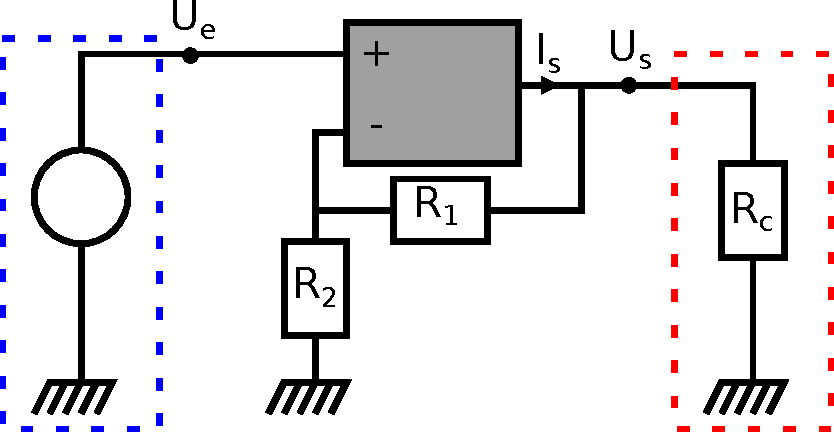
\includegraphics[width=0.5\linewidth]{puissance_AO.pdf}
\end{figure}

\newpage

\section*{Exercice 2}

On considère le montage suivant. L'AO est supposé idéal.

\begin{figure}[!h]
\centering
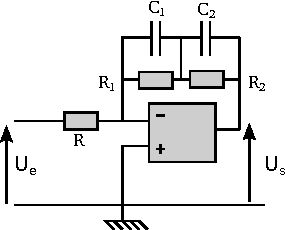
\includegraphics[width=0.5\linewidth]{circuit_6.pdf}
\end{figure}

\begin{itemize}

	\item[$\ast$] Déterminer la fonction de transfert de ce filtre, que l'on mettra sous la forme suivante : 
\begin{equation}
\underline{H}(j\omega) = H_{0}\frac{\prod_{k} (1+j\omega/\omega_{k})}{\prod_{l} (1+j\omega/\omega_{l})}
\end{equation} 

\item[$\ast$] Tracer le diagramme de Bode correspondant en fonction des différentes pulsations en jeu. Expliciter les cas possibles.

\item[$\ast$] On considère désormais que $R=R_1=R_2$ et $C_1=C_2=C$. Simplifier la fonction de transfert, en introduisant $\omega_0=1/RC$. A quel type de filtre à t-on affaire ?

\item[$\ast$] On envoie en entrée le signal suivant :
\begin{equation}
	U_e(t) = \frac{4U_0}{\pi}\sum_{p=0}^{\infty}\frac{1}{2p+1}\sin(2(p+1)\omega t)
\end{equation}
On suppose que $\omega\gg\omega_0$. Quel est le signal de sortie $U_s$ ? Donner son allure et commenter. 

\end{itemize}

 \newpage

\section*{Exercice 3}

On considère le filtre suivant :

\begin{figure}[!h]
\centering
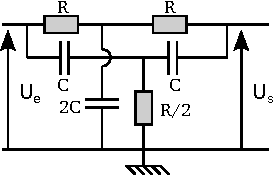
\includegraphics[width=0.5\linewidth]{circuit_2.pdf}
\end{figure}

\begin{itemize}

	\item[$\spadesuit$] Quel est le comportement de ce filtre à basse et haute fréquence ? 
	
	\item[$\spadesuit$] Montrer que la fonction de transfert peut s'écrire sous la forme :
	\begin{equation}
		H(x) =\frac{1+(jx)^2}{1+4jx + (jx)^2}
	\end{equation}
	où $x=\omega/\omega_0$ avec $\omega_0$ une pulsation que l'on déterminera. Tracer le diagramme de Bode correspondant. 
	
	\item[$\spadesuit$] Déterminer la bande "coupante" $\Delta\omega$, cad la plage de pulsations $\Delta\omega$ pour lesquelles $G^{dB}(\omega)\leq G^{dB}_{max} - 3$. On rappelle que $20\log\left( \sqrt{2}\right)\simeq3 $.
	
	\item[$\spadesuit$] On envoie le signal $U_e(t)=U_0\cos^3(\omega t)$ en entrée, avec $\omega=\omega_0/3$. Déterminer le signal de sortie $U_s(t)$. Tracer schématiquement les signaux.

\end{itemize}

\newpage

\section*{Exercice 4}
\begin{itemize}
\item[$\star$] Explicitez la fonction de transfert de ce filtre, puis calculez son gain et sa phase. On notera $\omega_0$ sa pulsation caractéristique. Quel est son rôle ?
\begin{figure}[!h]
\centering
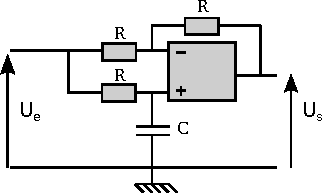
\includegraphics[width=0.5\linewidth]{circuit_.pdf}
\end{figure}

\item[$\star$]
Pour quelles conditions sur le circuit et le signal d'entrée trouve t-on que le circuit retarde un signal périodique sans le déformer, c'est-à-dire que $U_{s}(t)=U_{e}(t-\tau)$ ? Exprimez alors ce retard $\tau$ en fonction de $R$ et $C$.

On pourra utiliser la décomposition en série de Fourier du signal d'entrée :
\begin{equation}
U_e(t) = \sum_n C_n\cos(n\omega t + \varphi_n)
\end{equation}

\item[$\star$] On envoie en entrée le signal suivant :
\begin{equation}
U_{e}(t) = U_{0}\cos^{3}(\omega t)
\end{equation}

Décrire l'effet du filtre sur ce signal pour $\omega = \frac{\omega_{0}}{3}$ et $\omega=10^{-2}\omega_0$, et donner l'allure du signal de sortie. On donne $\arctan(1/3)\simeq\pi/10$.

\item[$\star$]
On suppose le condensateur déchargé à $t=0$. On envoie un échelon de tension $E$ en entrée. Quelle est la sortie ? Commenter.
\end{itemize}

\newpage

\section*{Exercice 5}

On considère le montage ci-dessous :
\begin{figure}[!h]
\centering
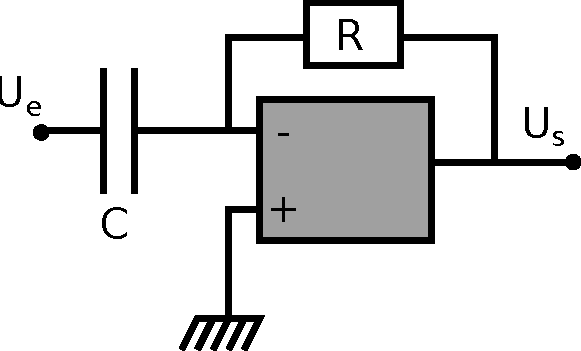
\includegraphics[width=0.5\linewidth]{derivateur.pdf}
\end{figure}
\begin{itemize}
	\item[•] On suppose dans un premier temps que l'AO est idéal. Qu'est-ce que cela signifie ? Calculez la fonction de transfert de ce montage. Quel est son rôle ?
	\item[•] On suppose désormais que l'AO est réel. On suppose alors que la sortie $u_s$ est reliée à $\varepsilon=u_+-u_-$ par la relation :
	\begin{equation}
		\tau\frac{du_s}{dt} +u_s = \mu_0\varepsilon
	\end{equation}
	avec $\mu_0=10^5$ et $\frac{\mu_0}{2\pi\tau}=$1MHz.
	
	Quel est la nouvelle fonction de transfert ? 
	
	Le montage est il stable ?
	
	\item[•] Que se passe t-il si l'on intervertit les bornes + et - de l'AO ?
	
	\item[•] A quel type de montage ce circuit s'apparente t-il ? Calculez ses caractéristiques pour $R=10$k$\Omega$ et $C=$100nF. Pour quelle fréquences agit-il comme un dérivateur ? 
\end{itemize}

\end{document}
